\documentclass[12pt]{article}

\usepackage[margin=1.5cm, top=1cm]{geometry}
\usepackage{amsmath, amsfonts}
\usepackage[version=4]{mhchem}
\usepackage{mathrsfs}
\usepackage{graphicx}
\usepackage{subcaption}
\usepackage{hyperref}
\usepackage{cite}
\usepackage{listing}
\usepackage{wrapfig}
\usepackage{graphbox}

\newcommand*{\figref}[2][]{%
  \hyperref[{fig:#2}]{%
    Figure~\ref*{fig:#2}%
    \ifx\\#1\\%
    \else
      \,#1%
    \fi
  }%
}

\begin{document}

\pagenumbering{roman}

\begin{titlepage}
    \begin{center}
        \vspace*{1cm}
 
        \textbf{Characterizing a Low Energy Electron Gun for use in Inverse Photoemission Spectroscopy}
             
        \vspace{1.5cm}
 
        \textbf{Michael Bouliane}
 
        \vfill
             
        A report submitted for partial fulfillment of the requirements of Phys 437B

        Source files and full sized images available at: \url{https://github.com/m-bouliane/Phys-437B}
             
        \vspace{0.8cm}
             
        Department of Physics and Astronomy\\
        University of Waterloo\\
        \today\\
             
    \end{center}
\end{titlepage}

\begin{abstract}
Inverse photoemission spectroscopy (IPES) provides a means to map the unoccupied electronic states of materials which are inaccessible to other techniques which map 
occupied electronic states. The coupling of electrons in an emitted beam to these unoccupied states can release detectable photons through the process 
of inverse photoemission. Unfortunately inverse photoemission spectrometers are not commercially available, and thus have to be built up from 
scratch. In order to obtain quality IPES results, a spectrometer has strict requirements for its electron source, photodetectors, and sample quality. 
This means that upon completing the construction of a spectrometer much work needs to be done to characterize its performance to ensure it is 
capable of collecting good data. 

Having previously focused on the photodetection capabilities of our spectrometer for Phys 437A, this report details our efforts to characterize our
electron source. Inverse photoemission requires low energy electrons, in a well collimated beam with a high brightness and small spot size. Space 
charge effects make this a very difficult task, which thankfully commercially available systems have solved for us. The task is to therefore find 
the appropriate operating conditions of the electron source which meet the above requirements, yet another difficult task due to the large parameter space
of the optimization problem.

By measuring the beam width and brightness at a set of manufacturer recommended parameters, we found a beam which was unfit for IPES applications. 
Space charge effects were found to be the limiting factor of this beam, so changes were made when exploring parameter space to minimize its impacts. 
Eventually a beam with a spot size of $2.033\pm0.014$mm and divergence angle of $4.15\pm0.50^\circ$ was obtained. The momentum resolution of the beam 
was then calculated to be $(1.07\pm0.13)\times10^9\mathrm{m}^{-1}$, an order of magnitude less than the size of copper's first brillouin zone. Our 
efforts to produce a beam fit for inverse photoemission spectroscopy were an overwhelming success, agreeing strongly with the results published by 
groups working with similar systems. 

Finally an angle resolved inverse photoemission experiment was performed on Cu(111), which did not at all meet expectations. We determined that 
this was due to sample quality and not the electron beam or photodetectors. Future tests on Cu(111) will be performed in an attempt to obtain results 
which align with those reported in literature, giving us vital insight into our spectrometer's overall performance.
    
\end{abstract}

\clearpage

\tableofcontents
\clearpage

\listoffigures
\listoftables

\clearpage

\pagenumbering{arabic}

\section{Introduction}
    Inverse photoemission spectroscopy (IPES) is an experimental technique used in condensed matter physics to map the unoccupied electronic structure
    of a material. In an ultra-high vacuum environment, a beam of electrons of known energy is impinged on a sample. If the energy of the incoming
    electrons align with a state which lies above the fermi energy, then they will couple to that state. Detections come from photons released through
    radiative relaxation of these excited states, which are in the UV range for typical electron energies of 10-100eV. We are able to map the unoccupied states
    by recording the number of photon detections we obtain at a given incident electron energy. In order to obtain significant IPES results a spectrometer must meet strict requirements of both its photodectors and its electron source. Our previous efforts in 
    spectrometer characterization focused on its photodetection capabilities. In this report we detail our work to characterize the performance 
    of our electron source.

    The electron source, also referred to as an electron gun, must be capable of operating within at low electron energies while still producing a beam with a minimal spot size and 
    momentum spread. The current of electrons reaching the sample should also be as large as possible, equivalent to the gun having a high brightness. Achieving this is a highly 
    non-trivial due to the contradictory requests of being low energy but also high brightness\cite{stoffel1985low}. Emission current limitations in these type of guns are caused by the space charge effect, 
    where the cloud of low energy electrons that make up the beam repel incoming electrons back towards the source\cite{staib}. Commercially available 
    electron guns are capable of meeting these requirements and thus solve the problem of needing to carefully balance these two main considerations; however they introduce a 
    new problem in that one is now tasked with finding the operating conditions of the gun which allows it to do so. The electron gun in our spectrometer has 10 unique parameters
    which can each be varied by applying a voltage bias. So to obtain a high brightness beam which operates at low energies we need to determine a combination of these 10 
    voltages, an optimization problem that is made exceedingly difficult by this large parameter space. 

    Starting with the configuration recommended by our electron gun's manufacturer we measured the beam width and maximum current. The beam was found 
    to be insufficient for use in IPES, which was attributed to space charge limiting. Reducing the temperature of the gun's cathode allowed us 
    to remove a parameter from the optimization problem, and yielded much better results in subsequent tests. Further constraints were placed on the 
    possible configurations which could use for the gun, which again reduced the difficulty of the optimization problem. Eventually a set of parameters 
    was found, which produced a beam of gaussian profile with a small spot size and divergence angle, on par with what has been reported by other groups\cite{ipes,raj2004optimization,stoffel1985low,budke}.
    Subsequent calculations showed that this beam is able to resolve the first brillouin zone of copper. Our spectrometer is now in a condition where 
    only minor work needs to be carried out before we are able to produce meaningful IPES results.


\section{Inverse Photoemission Spectroscopy}

\subsection{The Inverse Photoemission Process}

A useful way to understand inverse photoemission is to think of it in the context the photoelectric effect. Photons incident on the surface of a sample with a sufficiently
large energy will lead to the liberation of electrons. The determining factor in this process is if the photon has an energy greater than or equal to the sample's work function, which 
is defined as the energy difference between the sample's fermi level and vacuum level. The fermi level is the highest energy occupied electronic state, and the 
vacuum level is the energy of a free electron above the sample's surface. Inverse photoemission is the dual of this process, where instead a beam of electrons incident on a sample 
leads to the emission of photons through radiative decay. 

The mechanism through which this occurs starts with the electron coupling to an unoccupied electronic state with an energy that matches its initial energy, the state must be unoccupied in 
order to satisfy the Pauli principle. This unoccupied state is of a relatively high energy compared to the fermi energy, meaning that the sample remaining in this configuration 
is energetically unfavourable. As a result the electron decays to a lower energy unoccupied state, and the energy difference between the two states is what determines the energy of 
the emitted photon. It should be noted that at this electron energy range the penetration depth of electrons into a sample is at its minimum\cite{penn1987electron},
making IPES a very surface sensitive technique.

There are two ways to use this process for spectroscopy. In the first, the electron energy is varied and only photons of a single frequency are detected. 
In the second, the electron energy is fixed and the full range of emitted photons is collected. These modes are known as isochromat and spectrograph respectively; our system operates in the isochromat 
mode so we will limit the scope of further discussion to reflect this. 

\subsection{Energy Conservation in Inverse Photoemission}

In isochromat mode we vary the energy of electrons and record the intensity of photons with a set frequency $\omega_0$, thus the electron can only decay to states which meet the requirement that:

\begin{equation}
    E_i = \hbar\omega_0 + E_f
\end{equation}

Which means that if we know $E_i$ and $\omega_0$ then we can determine the energy of the unoccupied state $E_f$. So IPES allows us to map all of the $E_f$ states by varying $E_i$ and 
recording photon intensity. In general determining $E_i$ is a difficult task, since it is defined as:

\begin{equation}\label{vg}
    E_i = eV_g + \Phi_g
\end{equation}

where $V_g$ is the voltage applied to the electron gun's cathode, and $\Phi_g$ is the work function of the cathode. The difficulty comes from the fact that we don't know $V_g$ to great 
precision, and don't have a value for $\Phi_g$ at all. We can overcome this by measuring $E_f$ relative to the fermi energy, so for example if we get a peak in our spectrum at 
$E_f = 5\textrm{eV}$, then we know that there is an unoccupied state at an energy of 5eV above the fermi level. As we will later see however, 
this approach is insufficient if we want to perform what is called an angle resolved measurement on the sample. In this case we need to know the 
momentum of the electrons reaching the sample, and doing so requires a knowledge of the kinetic energy of the electrons which depends on $E_i$. 

\subsection{Momentum Conservation}

At the scale of an electron incident on a macroscopic sample, there is essentially infinite translational symmetry in the directions parallel to the sample's surface.
This symmetry means the electron's momentum in those parallel directions must be conserved as it changes from being a free electron to being bound 
in one of the sample's energy levels. This adds a further requirement that the momentum of the states to which the electron couples and decays into must match its initial parallel momentum. 
If we consider the kinetic energy of a free electron\cite{ipes}, just before it is bound to the sample we have:

\begin{equation}
    E_k = \frac{\hbar^2 k^2}{2m_e}
\end{equation}

Solving for the magnitude of the electron's momentum and we get:

\begin{equation}
    k = \frac{\sqrt{2m_e E}}{\hbar}
\end{equation}

If we define $\theta$ as the angle between the beam's axis and the samples surface, then the parallel component of the momentum is given by:

\begin{equation}\label{kpar}
    k_\parallel = k\sin{\theta}
\end{equation}

So by changing the incidence angle of the electron beam we are able to select states with the same $E_i$ value but with a different $k_\parallel$, letting us probe much more of 
the band dispersion. This technique is known as angle- or k-resolved inverse photoemission spectroscopy (KRIPES) and is one of the biggest selling points of the IPES method. 

\subsection{The Contact Potential}

Similarly to $E_i$, determining a value for $E_k$ is equally difficult since it is defined as:

\begin{equation}
  E_k = E_i - \Phi_s
\end{equation}

Where $\Phi_s$ is the work function of the sample undergoing inverse photoemission. If we insert equation \eqref{vg} we find that:

\begin{equation}
  E_k = eV_g + \Phi_g - \Phi_s
\end{equation}

We define the contact potential, $\Delta$, to be:

\begin{equation}\label{delta}
  \Delta = \Phi_s - \Phi_g
\end{equation}

Which tells us that the kinetic energy of the incident electrons is given by:

\begin{equation}\label{Ek}
  E_k = eV_g - \Delta
\end{equation}

Since $\Delta$ is dependent on the work function of the sample, its exact value will change for every sample we study with IPES. Determining a value for $\Delta$ can thankfully be
done by following a simple procedure\cite{mcmahon_2012}. With the electron beam incident on a sample with a known energy, we apply a bias voltage to the sample and record the 
resulting sample current. With an increasing sample bias, the current should remain mostly constant until reaching a threshold value where the current rapidly drops to zero. Keeping 
the sample bias voltage and gun cathode voltage in mind we consider the required $V_g$ to overcome the potential barrier created by having $\Phi_s > \Phi_g$:

\begin{equation}
  V_g = \frac{\Phi_s - \Phi_g}{e}
\end{equation}

If we now apply an arbitrary bias voltage to the sample the cathode voltage needs to increase to:

\begin{equation}
  V_g = V_s + \frac{\Phi_s - \Phi_g}{e}
\end{equation}

Inserting equation \eqref{delta} and solving yields:

\begin{equation}\label{vgvs}
  \Delta = e(V_g - V_s)
\end{equation}

Thus using the cathode voltage and the threshold bias voltage we recorded, we can determine the contact potential and from that determine the kinetic energy of the electrons in beam.

\section{The Electron Gun}

\subsection{Thermionic Emission}

The electron gun used in our spectrometer is a thermionic emission type. In this design, a heated cathode is used as the source of electrons. The 
high temperature of the filament allows for electrons in the cathode to be thermally excited to its vacuum level. Low work function cathodes 
are chosen to reduce the operating temperature needed to excite the same amount of electrons. In the case of our electron gun, this is achieved by 
using a BaO coated filament which has a lower work function than the same filament without a coating\cite{kimballphysics}. The current density 
emitted from the cathode at a temperate $T$ and work function $\Phi$ is given by Richardson's Law:

\begin{equation}\label{richardson}
  J = A_G T^2 \mathrm{e}^{-\frac{\Phi}{kT}}
\end{equation}

Where $A_G$ is the cathode material's Richardson constant. From this we see that emission current is inversely proportional to work function, and 
proportional to cathode temperature. Thus we can obtain a comparable current to a hot, high work function cathode using a colder and lower work function 
cathode. A gun operating at these reduced temperatures will have a longer cathode lifetime, and is generally referred to as being in the temperature limited 
mode.

\subsection{Space Charge Effect}

When working with low energy electron beams, the space charge effect has a much greater impact on maximum achievable beam currents than 
high energy counterparts\cite{staib,stoffel1985low,raj2004optimization}.
As electrons are emitted from the filament, they form a space charge which will eventually form the beam. As the charge of this distribution increases, 
its repulsive force can send electrons back to the filament. It can further prevent electrons from leaving the filament in the first place. The current 
density of a space charge limited cathode is given by Child's Law:

\begin{equation}
  J = K \frac{V_d^{3/2}}{d^2}
\end{equation}

Where K is a constant, $V_d$ is the potential difference between the cathode and anode, and $d$ is the cathode to anode distance.
We notice that unlike Richardson's law, there is no longer a temperature dependence for our current density, meaning that a space charge limited
beam is resistant to temperature fluctuations. However, space charge limiting only becomes a significant factor at high cathode temperatures, 
after the gun moves out of the temperature limited mode.

\clearpage
\subsection{Electron Gun Construction}

\begin{figure}[h!]
  \centering
  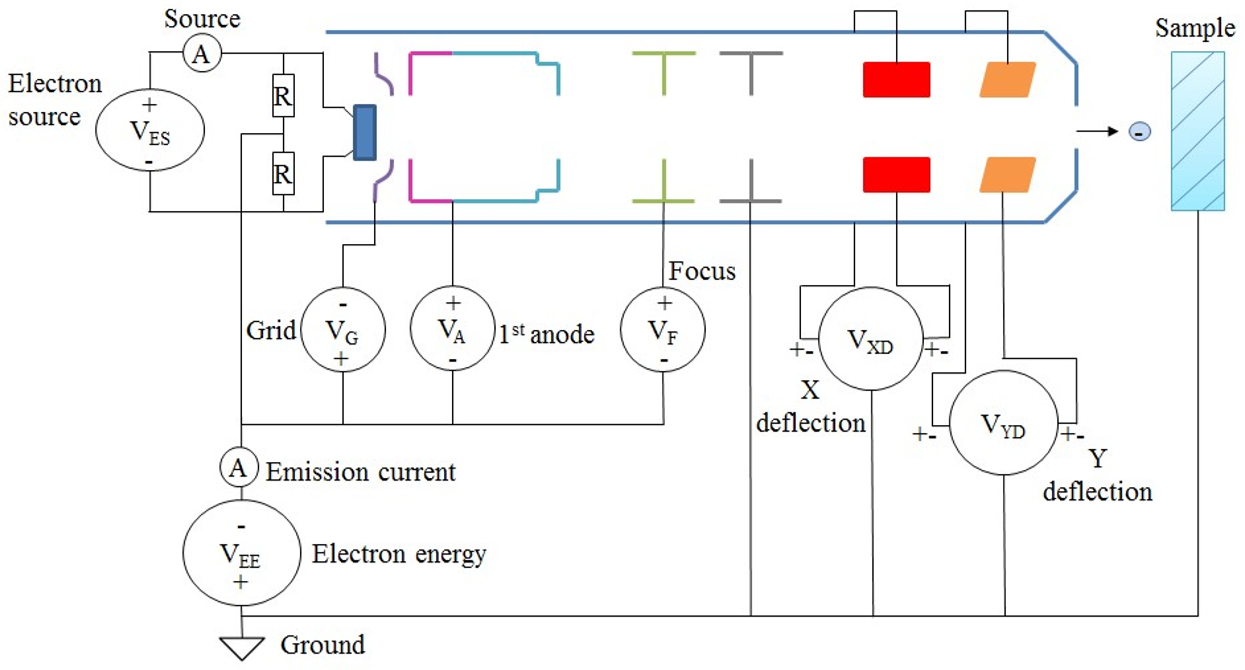
\includegraphics[width=0.85\linewidth]{../Assets/Gun diagram.png}
  \caption{Block Diagram of thermionic emission type electron gun for use in low energy applications\cite{gina_2012}}
  \label{fig:egun}
\end{figure}

Figure \ref{fig:egun} shows a typical design for low energy electron guns which use a heated cathode. The ground of the electron gun is connected 
to the supply which controls electron energy, meaning that all potentials are going to be floated by whatever potential is selected for electron energy. 
The sample and gun assembly share the same ground, meaning that the gun's potentials are also floating with respect to the sample. 

The filament supply voltage controls the temperature of the cathode, and is limited to a range of 0V to 5V. The temperature is increased through ohmic heating and an emission 
current is generated through thermionic emission. The electrons are accelerated through the gun by the extraction potential (labeled first anode in figure \ref{fig:egun}),
which is limited to a range of 0V to 100V. After being pulled from the cathode the electrons pass through the grid, which controls the brightness of the beam. 
It can be biased with a potential between -15V and 15V, a sufficiently negative grid voltage can suppress the emission of electrons entirely. The shaping
of the beam is done by the focusing electrodes. Our gun has two separate electrodes which can be independently biased in a range determined by the electron 
energy and extraction potential. Finally, the beam can be steered in the two directions perpendicular to its axis by using two parallel plate deflectors. 
This can be used to realign the beam towards the sample if it is found to be deflecting off target. 

The goal in characterizing an electron gun is to find a combination of all of these parameters which meet the strict requirements of inverse 
photoemission. A notable thing to balance is the cathode temperature and extraction voltage, as it controls if the gun is operating in the temperature limited 
or space charge limited regime. In the temperature limited regime we have longer filament lifetimes and a potential for larger sample currents, but 
the emission current is highly dependent on cathode temperature. Space charge limiting provides us stability in emission current but at the cost of 
a hot filament with a much lower lifetime and maximum emission. Best results are obtained when there is some balance between the two, yielding a stable and sufficiently high 
emission current, while also prolonging cathode lifetime\cite{stoffel1985low,staib}. Other considerations include keeping the focus potential to roughly the same order as the extraction 
potential, which minimizes the amount of accelerating and decelerating an electron in the beam undergoes, which is more likely to provide a well 
behaved beam\cite{stoffel1985low,raj2004optimization}.
\section{Experimental Design}

\subsection{Sample Preparation}

The sample used in this experiment is the same one which was used in the Phys 437A project. For the sake of brevity this section will serve only as a review of the sample preparation procedure. 

A Copper single crystal with dimensions 10mm $\times$ 10mm $\times$ 1mm was chosen for the experiment, with the $[111]$ direction being normal to the sample's surface. The sample was 
cleaned chemically first using a dilute acid wash, followed by cleaning with a series of organic solvents. The sample was transferred to the prep chamber of our spectrometer and 
cycled through Argon ion etching and annealing at $400^\circ$C\cite{robinson2012argon} until the resulting low energy electron diffraction pattern was sharp and well ordered. 

After completing the Phys 437A project the sample was left in the spectrometer's IPES (main) chamber under high vacuum conditions, being exposed to pressures no higher than $9\times10^{-10}$ torr.


\subsection{The IPES Chamber}

The experiment was conducted within the IPES vacuum chamber portion of our spectrometer. Within the chamber is a motorized sample holder with the ability to translate along $x$, $y$ and $z$ 
directions, with $z$ denoting the central axis of the chamber. A design diagram is presented in figure \ref{fig:holder}. The holder is also capable of rotation about the $z$ axis with the rotation angle denoted $\theta$. A sample can be
secured to this holder which allows for it to be positioned in the output of the electron gun. The current from the electron gun can be measured as the total current reaching the 
sample, or as the current at a certain location in space using a Faraday cup mounted above the sample. A Faraday cup is a conductive cup with a pinhole sized opening, meaning only the portion 
of the beam which intersects the pinhole will contribute to the current measurement. Keithley Instruments 6485 and 6487 picoammeters are used to record these currents, which are connected to 
the chamber using coaxial cable vacuum feedthroughs. The sample and Faraday cup share a common ground and can be biased to positive or negative potentials using the Keithley 6487's
voltage supply. This setup allows for high accuracy measurements of both the beam intensity and shape, and determining the sample's contact potential.

\begin{figure}[h!]
    \centering
    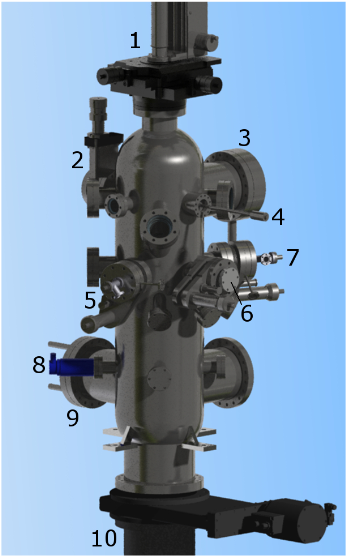
\includegraphics[scale=0.35]{../Assets/IPES.png}
    \hfil
    \includegraphics[scale=0.35]{../Assets/sample holder.png}
    \caption{Left: Diagram of IPES chamber showing the manipulator stage (1), electron gun (6), photodetectors (5, 7), and cryopump (10). 
    Right: Sample holder diagram, showing relative position of mounted sample (orange) and faraday cup. Coordinate axes indicate translational directions
    and direction of increasing $\theta$ can be seen\cite{mcmahon_2012}.}
    \label{fig:holder}
\end{figure}

\clearpage
The electron gun in our system is a commercially available design produced by Staib Instruments. The specific model, NEK-150, is reported to achieve a current of 5$\mu$A and a spot size of 1mm at electron 
energies below 10eV\cite{staib}. 

These devices are all interfaced to a computed through a labVIEW control program. It is capable of recording the current readings from the ammeters, setting the bias voltage applied 
to the sample and faraday cup, and controlling the electron gun. Custom scanning programs can be written to vary instrument parameters and record resulting measurements. 

\subsection{Procedure}

The desired operating parameters for the gun are fist set using the labVIEW control program. For contact potential and energy resolution determination, the sample is maneuvered in front 
of the electron gun at a set working distance. The Keithley 6487 is used to bias the sample over a set range of voltage values with a given voltage increment. At each step of increasing 
the bias the sample current is recorded, also done using the 6487 picoammeter. The Faraday cup can be used instead of the sample itself if the goal is to observe the energy distribution 
of the beam at specific locations. 

Measuring the width of the beam is done using the Faraday cup. The cup is aligned with the beam, and then translated along a direction perpendicular to the beam's axis. For most 
runs in this experiment the direction chosen was the $x$ direction, with the beam aligned along the $y$ direction of figure \ref{fig:holder}. Once the Faraday cup is translated completely 
out of the beam, a scan is started to increment its position such that it traverses across the entire beam. At each position the picoammeter records the current of the beam, as well 
as the position readout from the motor's rotary encoder. It will be seen in the results that the absolute position values across different measurements 
can vary significantly. The reason for this is a reset of the motor position, with zero representing the position of the motor on start up. This has no effect on the results presented since only 
relative distances are important for any calculations, and any qualitative behaviour can be understood by using the coordinate axes of the spectrometer.

The above procedure can be further expanded by adding an additional scanning direction. Allowing the Faraday cup to scan in the $z$ direction as well as the $x$ direction will create a 
raster scan. This is particularly useful to gauge the symmetry of the beam, since a while behaved beam should be rotationally symmetric about its axis. If instead the Faraday cup is 
moved in a combination of $y$ and $x$ directions the beam width at different working distances can be found. This allows for the beam's divergence angle to be computed, which can be 
used to determine the broadening in the beam's momentum distribution. 

Finally, KRIPES measurements are taken by setting an incidence angle, $\theta$, using the rotational motor. The photodetectors are then filled with acetone to the appropriate pressure, and 
the corresponding high voltage is applied to the anode wire. The photodetector configurations were determined previously through experiment in Phys 437A. 
The electron gun sweeps through a set range of $E_i$ values and records the number of detections which come from the photodetectors. 
The incident angle can be varied and the scan repeated to show how the unoccupied states change with momentum. 

The process of characterizing the electron gun involved examining a wide range of operating parameters and testing the beam's performance using the first two experiments. Once a 
good configuration was found it was further studied using raster scans and longitudinal scans. The fully characterized beam was finally used for a series of k 
resolved inverse photoemission measurements, which could then be compared to results reported in literature. 
\section{Results}

\subsection{Unoptimized Beam}

The experiment to determine the contact potential of the sample-gun system can be performed using any configuration for the gun and in a very short 
amount of time. The utility of the contact potential made this the most logical first step. By setting $V_g$ to 15V and biasing the sample 
from 0V to 20V, we obtain the results shown in Figure \ref{fig:contact}. This measurement was repeated a total of three times. 
The value $V_s$ is determined by finding the first bias voltage at which the sample current begins to increase, and it was found to be 
$8.37\pm0.05$V. Recalling equation \eqref{vgvs} we find that the contact potential for this specific system is $\Delta = 6.63\pm0.05$eV.

\begin{figure}[h!]
	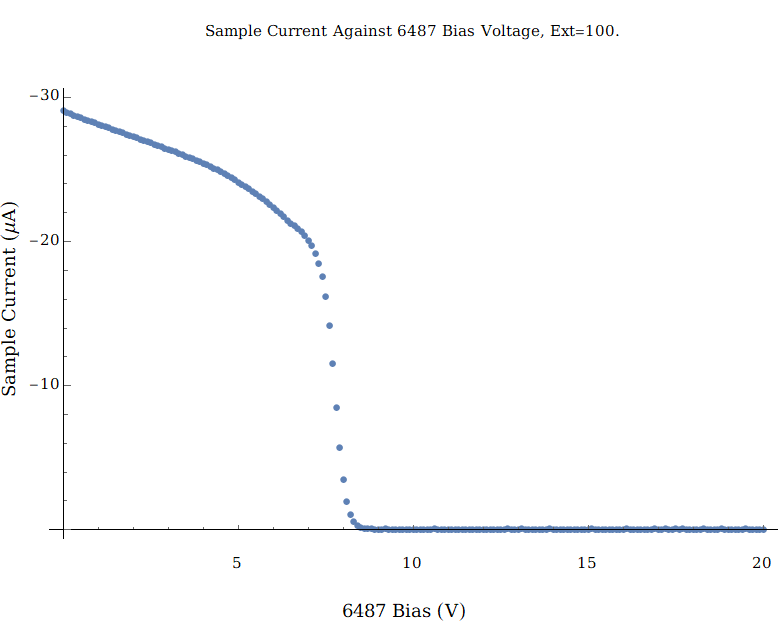
\includegraphics[width=0.32\linewidth]{../Test Scans/GunResPlots/Plot1_Ext100.GunResTest.png}
	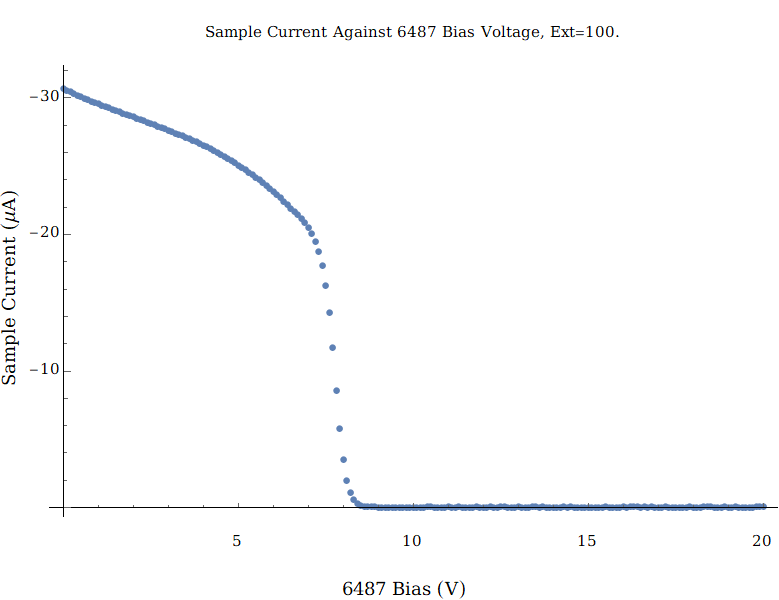
\includegraphics[width=0.32\linewidth]{../Test Scans/GunResPlots/Plot2_Ext100.GunResTest.png}
	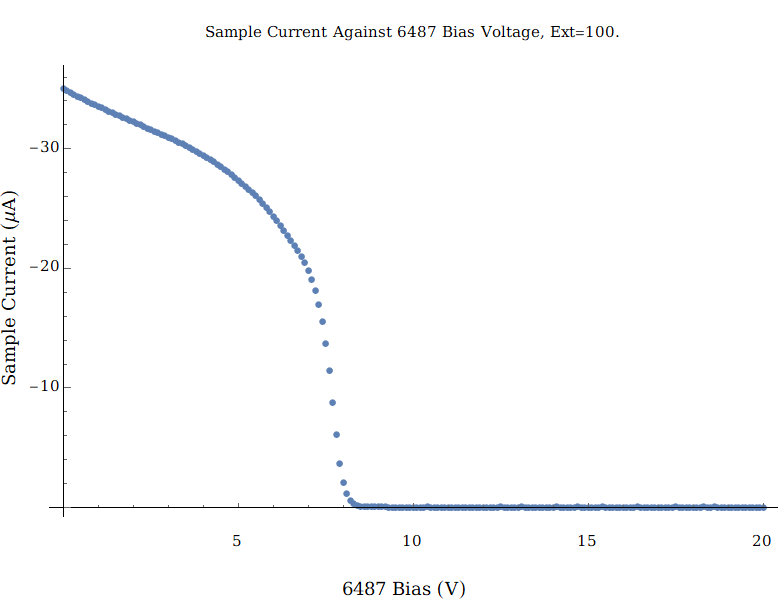
\includegraphics[width=0.32\linewidth]{../Test Scans/GunResPlots/Plot3_Ext100.GunResTest.png}
	\caption{Sample current against sample bias voltage for contact potential determination}
	\label{fig:contact}
\end{figure}

Unlike determining the contact potential, the process of finding optimal values from a parameter space this large is a challenging task. Thankfully the manufacturer of the electron gun used provided a list of starting parameters
which were recommended for an electron energy of 15eV. With the values in table \ref{tab:recpar} applied to our gun, we started by measuring its width along both the $x$ and 
$z$ directions. The beam was found to be roughly 15mm wide in both directions, an order of magnitude too large for use in IPES. Further we see that the beam appears to be more 
concentrated towards its edge, meaning that at this configuration the beam is poorly collimated in addition to being too large. 

\begin{table}[h!]
	\centering
	\begin{tabular}{ccccccc}
		\hline
		\multicolumn{1}{l|}{Paremeter} & Filament* & Energy & Extraction* & Grid & Focus 1 & Focus 2 \\ \hline
		\multicolumn{1}{l|}{Value (V)} & 5.0 & 15.0 & 100.0$\rightarrow$50.0 & -13.4 & 8.0 & -9.3 \\ \hline
	\end{tabular}
	\caption{Starting parameters recommended by Staib Instruments for the NEK-150 low energy electron gun at $E_i=15$eV. A recommended filament 
	voltage was not provided, so it was chosen arbitrary. Finally, using the recommended extraction value of 100V was not possible since it caused 
	the emission current of the gun to exceed its safe maximum value. To protect the filament we had to turn the extraction down to 50V.}
	\label{tab:recpar}
\end{table}

\begin{figure}[h!]
    \centering
    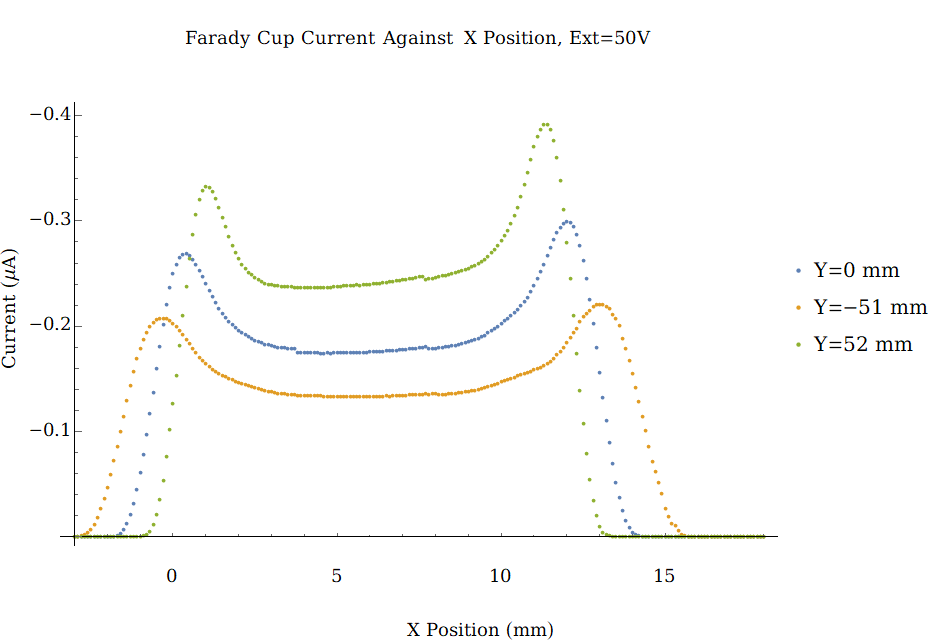
\includegraphics[width=0.45\linewidth]{../Test Scans/GunResPlots/BeamWidthXVaryingYExt50.png}
	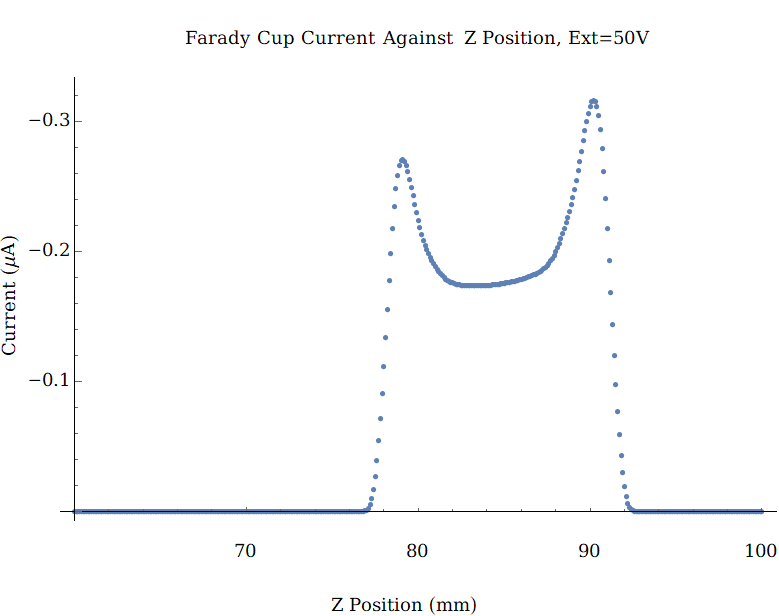
\includegraphics[width=0.45\linewidth]{../Test Scans/GunResPlots/BeamWidthZExt50.png}
	\caption{Beam width measurements taken using recommended operating parameters. Left: Beam current against $x$ position at different working distances. Increasing $y$ position is closer to output of electron gun. 
	Right: Beam current against $z$ position, at fixed working distance}
    \label{fig:badbeam}
\end{figure}

In order to corroborate these observations of an unexpected beam shape, we focused the Farady cup at three specific regions of interest within the beam.
At the left peak ($x=1$mm), the beam centre ($x=6$mm), and the right peak ($x=13$mm) we biased the cup with a potential ranging from 0V to 20V to probe the 
beam's energy spread. The results in figure \ref{fig:enres} show that the electrons at the beam's edge are easily repelled by small voltage 
biases. Comparing this to the electrons at the centre of the beam and we find that the current remains constant for increasing bias until reaching the 
threshold value where it quickly drops to zero. So while the beam has a higher concentration of electrons towards its edge, the energy distribution 
is more broad than at the beam's centre and thus contains a higher proportion of low energy electrons. 

\begin{figure}[h!]
    \centering
    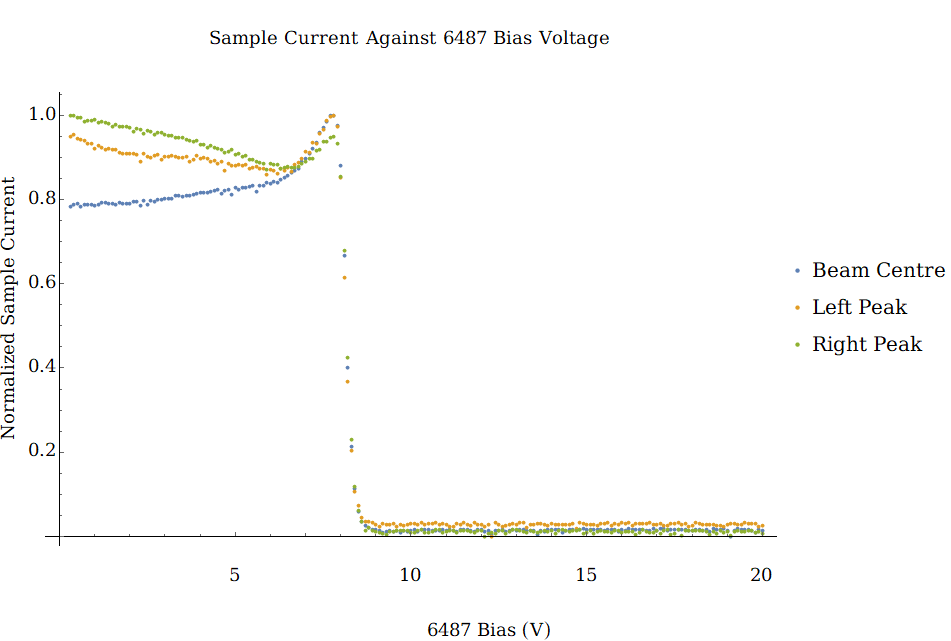
\includegraphics[width=0.85\linewidth]{../Test Scans/GunResPlots/ContactPotentialLocationsInBeam.png}
	\caption{Current of electron beam against Faraday cup bias voltage, for beam set to recommended operating conditions. The three locations correspond to 
	the features shown in figure \ref{fig:badbeam} and are at $x$ positions of 6mm, 1mm, and 13mm in order of appearance in plot legend.}
    \label{fig:enres}
\end{figure}

After obtaining these results we shifted focus to prioritize obtaining a gaussian beam profile above every other requirement. Referring back to 
table \ref{tab:recpar} we see that the filament voltage was the only free parameter we had when using the manufacturer recommended values. For simplicity
we chose the maximum value of 5V, which means the cathode is operating at its highest temperature. We hypothesized that at this high temperature, 
the broadened thermal energy distribution of electrons emitted from the cathode could lead to the broadening of the beam's shape and an excess of 
low energy electrons towards the beams edges. This hypothesis was tested by decreasing the filament voltage to lower the cathode's temperature.

\subsection{Lowered Temperature}

Our first test used a filament voltage of 4.5V, which allowed us to increase the extraction to the recommended 100V. 
Figure \ref{fig:firstgauss} shows that in this new configuration we do manage to obtain a gaussian profile, 
though its FWHM is roughly 8mm which is far too large for IPES. The discontinuities in the plot were caused by a loose backlash screw in the 
motor assembly, which was later fixed.

\begin{figure}[h!]
    \centering
    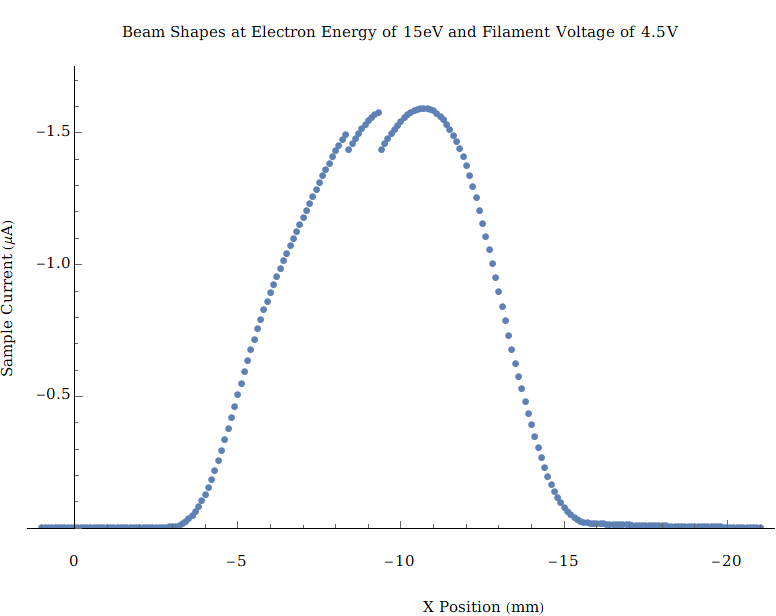
\includegraphics[width=0.85\linewidth]{../Work Term Replication/Plots/Work Term Replication E15Fil4.5.png}
	\caption{Beam current against Faraday cup $x$ position for reduced filament voltage of 4.5V, all other parameters remained unchanged from 
	table \ref{tab:recpar}.}
    \label{fig:firstgauss}
\end{figure}

While it is true we were able to increase the extraction to 100V, this configuration was not stable and the emission current slowly grew until it 
reached the maximum safe value of 100$\mu$A. Decreasing the filament voltage to 4V allowed for the beam to be operated at 100V extraction indefinitely. This was 
the filament voltage we decided to use for the remainder of the optimization. To make quicker work of this optimization problem we chose to alter the 
remaining values in large steps, exploring a wide range of parameter space. Similarly designed electron guns report achieving good performance when
the focus potential is roughly comparable to the extraction potential\cite{stoffel1985low,raj2004optimization}. This allowed us to limit our search even further by placing more emphasis 
on beam configurations where $F_1$ or $F_2$ were 100V. Figure \ref{fig:workterm} shows the beam widths at eight different configurations.

\begin{figure}[h!]
    \centering
    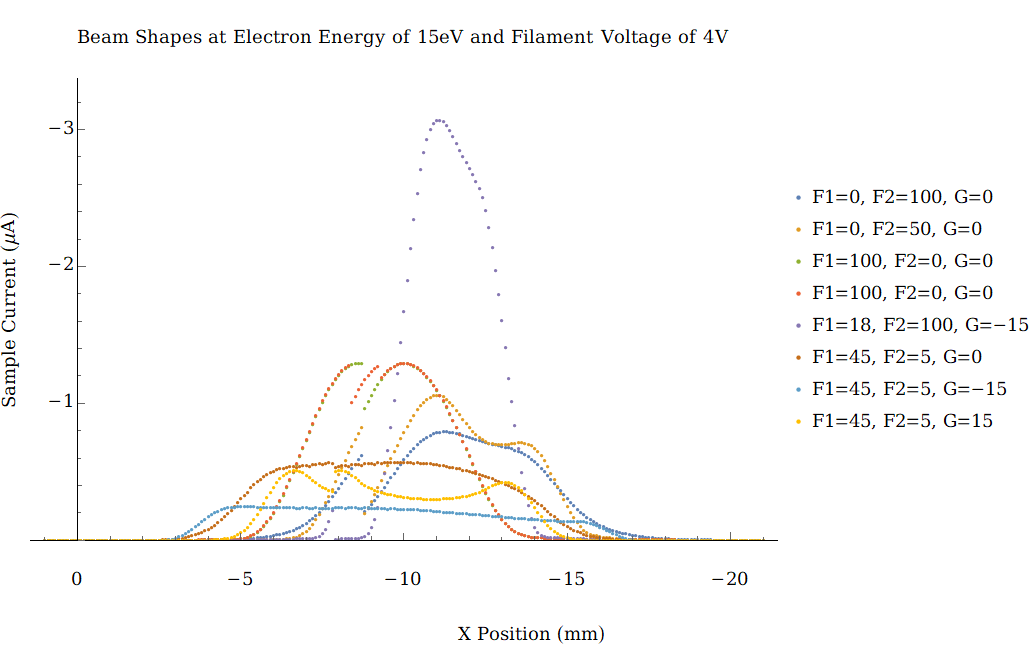
\includegraphics[width=0.85\linewidth]{../Work Term Replication/Plots/param sweep.png}
	\caption{Beam widths for varying $F1$, $F2$, and $G$ values at fixed $E_i=15$eV, $F=4$V and Ext$=100$V.}
    \label{fig:workterm}
\end{figure}

Standing out from all of the other configurations is one which has both the largest maximum current and the smallest beam width. The parameters 
used to create this beam are shown in table \ref{tab:optparam}. With this beam appearing to meet all of our requirements for inverse photoemission, 
we chose to characterize it further to see what improvements could be made.

\begin{table}[h!]
	\centering
	\begin{tabular}{ccccccc}
		\hline
		\multicolumn{1}{l|}{Paremeter} & Filament & Energy & Extraction & Grid & Focus 1 & Focus 2 \\ \hline
		\multicolumn{1}{l|}{Value (V)} & 4.0 & 15.0 & 100.0 & -15.0 & 18.0 & 100.0 \\ \hline
	\end{tabular}
	\caption{Gun parameters used to obtain the large, narrow beam shown in figure \ref{fig:workterm}}
	\label{tab:optparam}
\end{table}

\clearpage
\subsection{Characterizing the Optimized Beam}

The divergence angle of a beam can be used to determine the parallel component of a beam's momentum, making it a vital quantity to calculate if 
one wants to characterize an electron beam for inverse photoemission. To accomplish this, a longitudinal scan along the beams axis was conducted, 
measuring its width at varying working distances. Figure \ref{fig:long} shows the hyperbolic profile of the beam made up of individual beam width 
scans at set $y$ positions. 

\begin{figure}[h!]
    \centering
    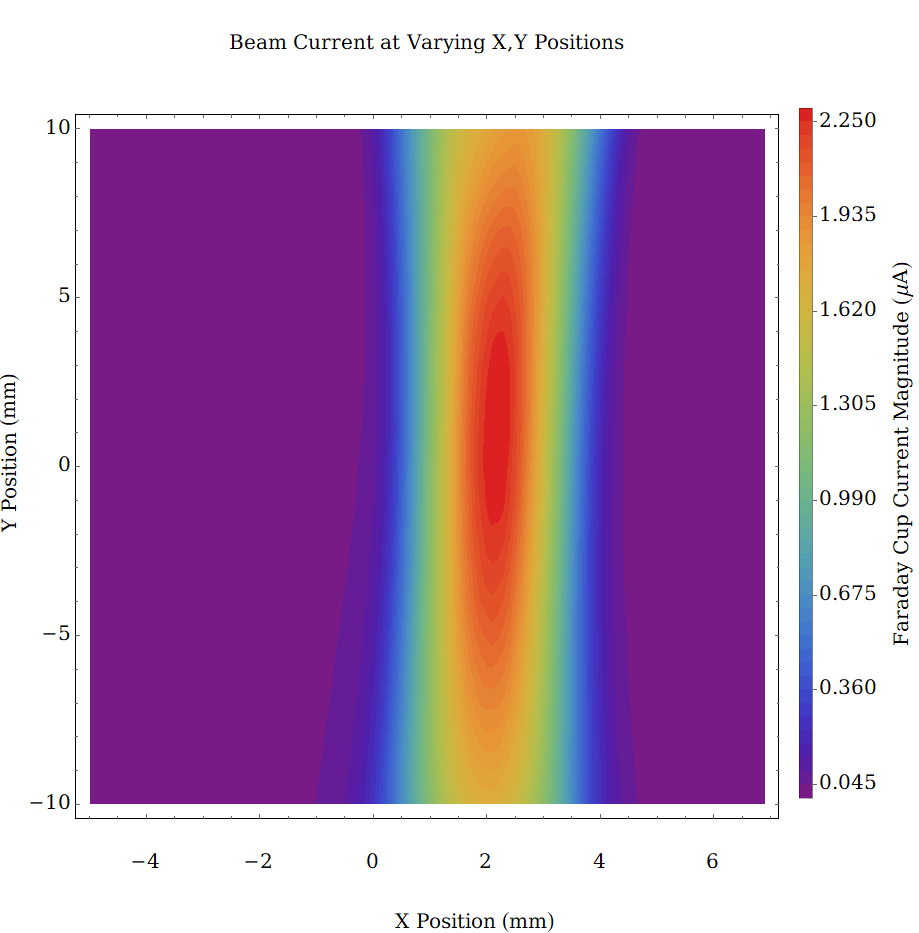
\includegraphics[width=0.85\linewidth]{../Beam Divergence/Plots/BeamwidthContour.png}
	\caption{Beam width as a function of distance along beam axis}
    \label{fig:long}
\end{figure}

A general gaussian of the form:

\begin{equation}
	I(x) = a \exp{\left(-\frac{(x-b^2)}{2c^2}\right)}
\end{equation}

was fitted to the current-position data. The full width at half maximum (FWHM) was used as the beam's width, and it is found using:

\begin{equation}
	\mathrm{FWHM} = 2\sqrt{2\ln2}c
\end{equation}

Figure \ref{fig:FWHM} shows how the FWHM changes along the beam's axis. 

\begin{figure}[h!]
    \centering
    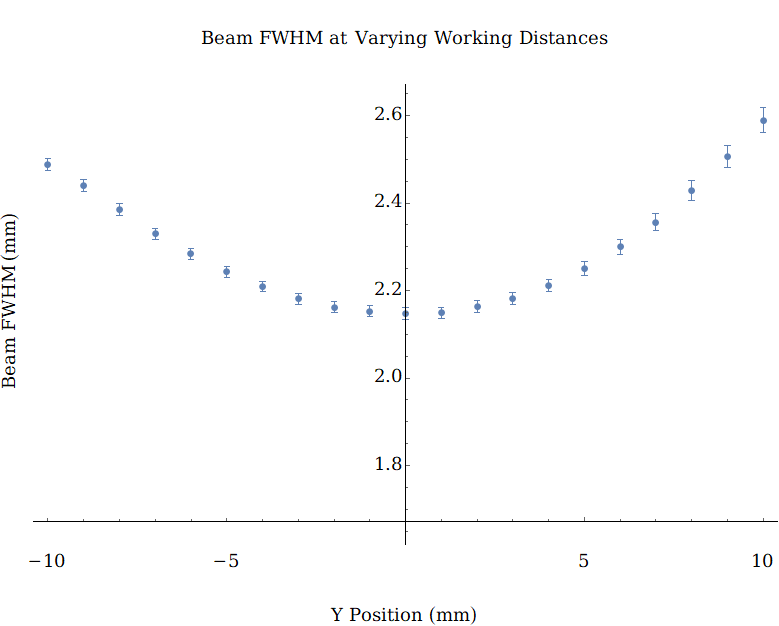
\includegraphics[width=0.85\linewidth]{../Beam Divergence/Plots/FWHM plot.png}
	\caption{FWHM as a function of distance along beam axis. Uncertainty was estimated using the standard deviation of fit parameters}
    \label{fig:FWHM}
\end{figure}

The divergence angle of a gaussian beam, $\Theta$, can be found using:

\begin{equation}
	\Theta = 2\arctan\left(\frac{D_f - D_i}{2\ell}\right)
\end{equation}

Where $D_f$ and $D_i$ are two separate beam diameters far from the beam's focus, and $\ell$ is the distance separating them. Using this the beam 
divergence angle was found to be $4.15\pm0.50^\circ$. 

As a final beam width scan, we can perform a raster in $x$ and $z$ to get a qualitative sense of the beams axial symmetry. The results of this 
are presented in figure \ref{fig:raster}.

\clearpage
\begin{figure}[h!]
    \centering
    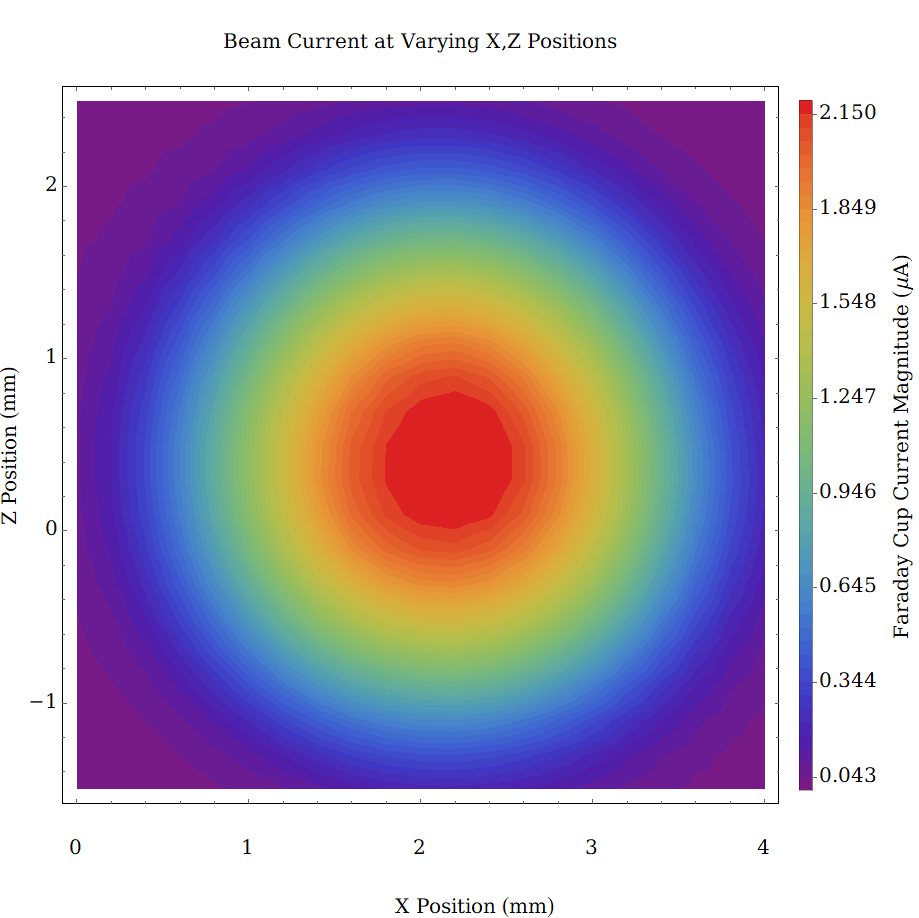
\includegraphics[width=0.85\linewidth]{../Beam Divergence/Plots/Raster plot.png}
	\caption{Raster scan of beam width in $x$ and $z$ directions, beam axis ($y$) is pointing into page.}
    \label{fig:raster}
\end{figure}

Finally, taking the derivative of equation \eqref{kpar} gives us the momentum resolution of the beam, $\Delta k_\parallel$, at an incidence angle $\theta$:

\begin{equation}
	\Delta k_\parallel = \frac{\sqrt{2m_e(E_k-\Delta)}}{\hbar}\cos\theta \Delta\theta
\end{equation}

Since the experiments were conducted at normal incidence we have $\theta=0$, and the angle broadening being given by $\Delta\theta = \frac{\Theta}{2}$.
From this we find the momentum spread of the beam to be\\$\Delta k_\parallel = (1.07\pm0.13)\times10^9\mathrm{m}^{-1}$.  

% \clearpage
\subsection{KRIPES Test on Cu(111) Single Crystal}

After finding a beam which met the criteria for inverse photoemission spectroscopy, and having previously characterized the system's photodetection
capabilities, we decided that as a final test we would attempt a k-resolved measurement of Cu(111). In inverse photoemission spectroscopy there 
are several samples which have been widely reported on in literature and serve as benchmarks spectrometer performance. One such example is the 
Cu(111) L-gap surface state, reported on by Budke et al. \cite{budke}, with expected results shown in figure \ref{fig:budke}. The state has a parabolic 
dispersion in $k_\parallel$, and appears as a peak roughly 0.25eV above the fermi energy. The L-gap state intensity grows sharply after an incidence angle 
of roughly $6^\circ$. 

\begin{figure}[h!]
	\centering
	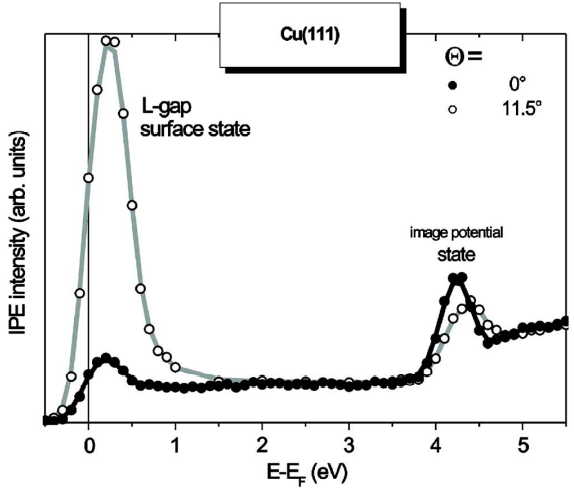
\includegraphics[width=0.45\linewidth, align=c]{../Assets/budke.png}
	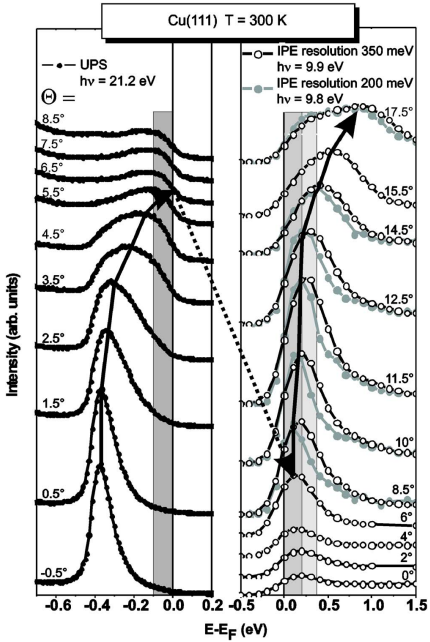
\includegraphics[width=0.45\linewidth, align=c]{../Assets/budke2.png}
	\caption{Left: K-resolved inverse photoemission spectra of Cu(111) at incidence angles of $0^\circ$ and $11.5^\circ$. Right:
	K-resolved measurements of L-gap state on Cu(111) (right subfigure) showing parabolic $k_\parallel$ dispersion\cite{budke}}
	\label{fig:budke}
\end{figure}

To replicate this we varied $E_i$ from 10eV to 20eV and recorded the resulting photon intensity. After a scan was completed, the incidence angle $\theta$
was varied using the rotational motor and another scan was performed. A selection of the spectra gathered is presented in figure \ref{fig:ipes}. 
Unfortunately no surface state was visible in the results, and an incident which ocurred later on left the sample in a state unfit for future trials. 

\clearpage
\begin{figure}[h!]
	\centering
	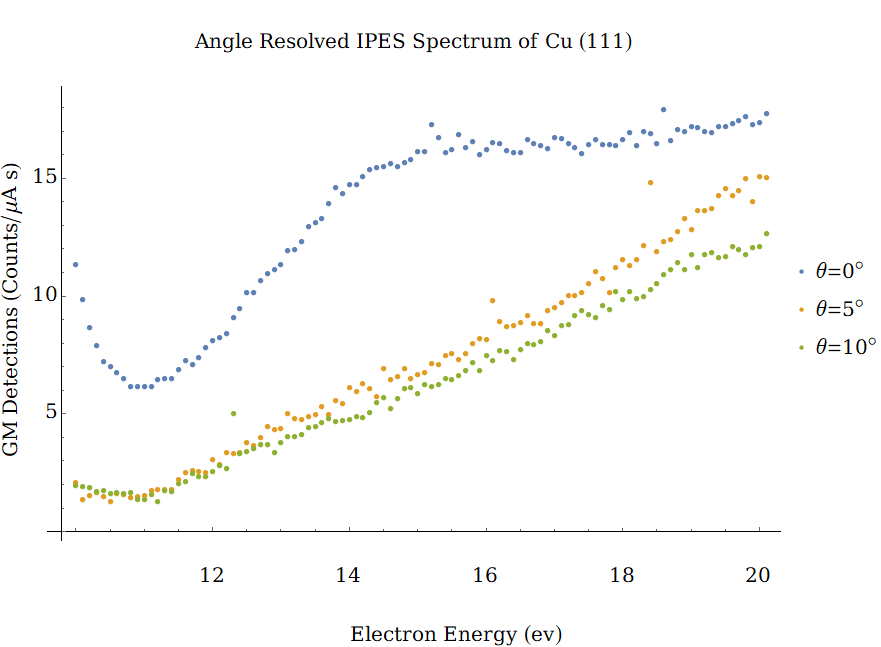
\includegraphics[width=0.85\linewidth]{../Cu 111 ARIPES/Plots/Better angle resolved.png}
	\caption{KRIPES of Cu(111) single crystal at incidence angles of 0$^\circ$, 5$^\circ$, and 10$^\circ$}
	\label{fig:ipes}
\end{figure}
\section{Discussion}

\subsection{Poor Performance of Recommended Parameters}

We had hypothesized that the strange beam shape and low sample current were caused by the filament being too hot. With the cathode voltage being at 
its maximum value, this was most likely placing the beam in a space charge limited configuration. One can see that the maximum observed current in 
figure \ref{fig:badbeam} was just $0.4\mu$A, which is an entire order of magnitude lower than the maximum current observed in the optimized beam. 
This has all of the characteristics of a space charge limited beam, meaning that the high temperature was indeed why we were not getting a well 
behaved beam. 

Explaining the observed shape is slightly more challenging. Stoffel and Johnson\cite{stoffel1985low} provide a figure (fig. \ref{fig:cath}) in their work outlining their gun design
that examines how cathode temperature affects beam emission. At a low temperature electrons emitted from the cathode's surface and passing through 
an aperture form a diverging beam with a single apparent source within the cathode. At an increased temperature, the thermal energy distribution is 
broadened and so the resulting beam appears to come from multiple source points withing the cathode. Our space charge limited beam can be described by 
the second case. The beam is broader than that of the low temperature cathode, and there are multiple points of overlap from the apparent sources. It 
is possible that the regions of overlap, after going through the electron optics, were focused to the beam's edge. This would explain both why there 
was a higher current at the edge, and why the electrons located there were at a lower energy then the electrons at the centre. 

\begin{figure}[h!]
    \centering
    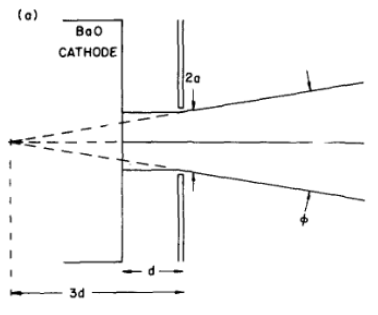
\includegraphics[width=0.45\linewidth]{../Assets/Low Temp.png}
    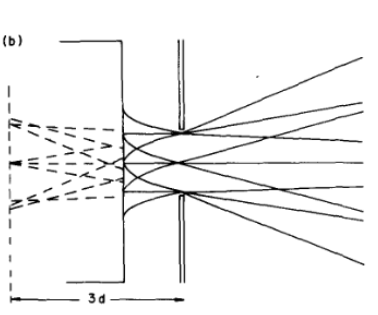
\includegraphics[width=0.45\linewidth]{../Assets/High Temp.png}
    \caption{Left: Emission from cathode operating in temperature limited mode. The dotted line indicate the apparent point source of the electron 
    beam, located within the cathode. Right: Emission from high temperature, space charge limited cathode. The widened beam now appears to come 
    from multiple apparent point sources\cite{stoffel1985low}}
    \label{fig:cath}
\end{figure}

\subsection{Optimized Beam Performance}

Our beam has a minimum FWHM of $2.148\pm0.013$mm, though as is stated in \cite{raj2004optimization} this is not truly indicative of the beam's spot size. 
Instead this represents a convolution of the beam's true gaussian profile with a rectangular function which reflects the aperture of the Faraday cup.
To find the true width of the beam, we convolve a boxcar function with a 1mm width (the size of the Faraday cup opening), with a general gaussian function. 
By then performing a non-linear fit of this convolution function to the minimum beam width data we are able to find a more representative FWHM for 
our beam, see figure \ref{fig:convolution}. We obtained a result of $2.033\pm0.014$mm, smaller than obtained from the raw data and in strong agreement with the results obtained by other 
groups\cite{raj2004optimization,ipes,Ciccacci}. These groups also report divergence angles in the range of $3^\circ$ to $7^\circ$, which our value 
of $4.15\pm0.50^\circ$ falls on the low end of. All of these groups have managed to publish novel and high quality results, indicating a strong 
future for our spectrometer once final characterization is complete.

\begin{figure}[h!]
    \centering
    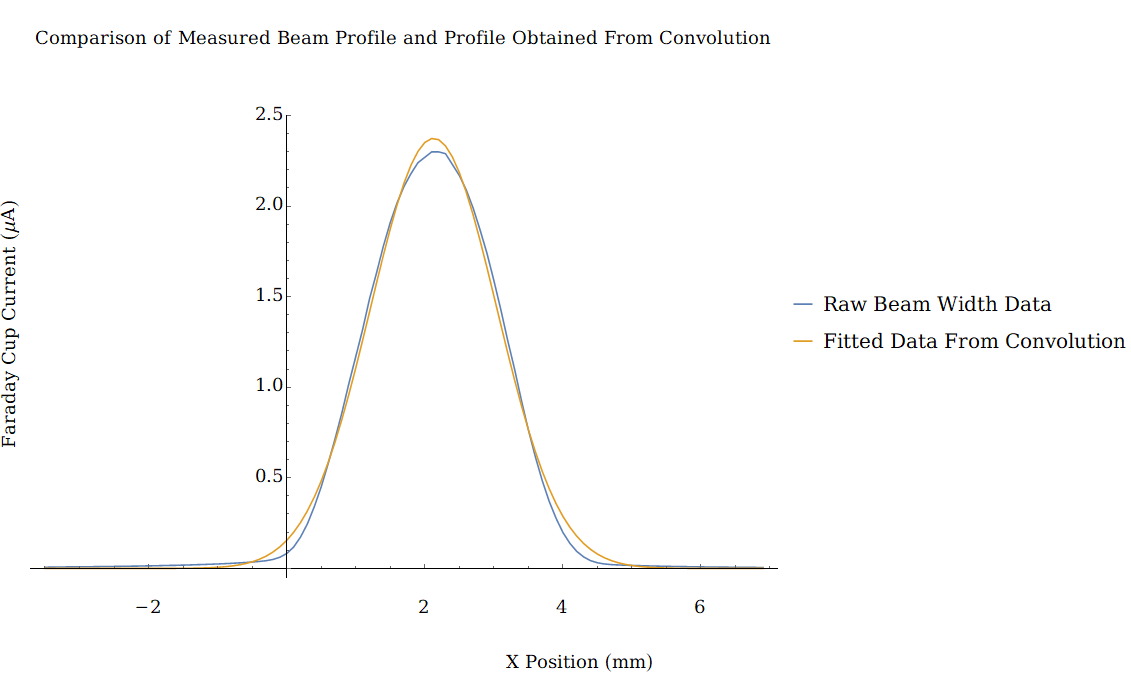
\includegraphics[width=0.85\linewidth]{../Beam Divergence/Plots/Convolution.png}
    \caption{Comparison of raw beam width data to the curve produced by convoluting a 1mm boxcar with a general gaussian function, and performing 
    a non-linear best fit.}
    \label{fig:convolution}
\end{figure}

We were able to use the divergence angle to calculate a momentum resolution of our beam, which we found to be $(1.07\pm0.13)\times10^9\mathrm{m}^{-1}$. 
If a beam's momentum resolution is too large, we will be unable to resolve fine details in the electronic structure of samples we are studying. 
A good way to put the value for $\Delta k_\parallel$ into context is to compare it to the size of the first brillouin zone of copper. Copper has 
an FCC unit cell, with a lattice constant, $a$, of 361.49pm\cite{reference.wolfram_2021_elementdata}. The size of the brillouin zone is given by:
\begin{equation}
    d = \frac{2\pi}{a}
\end{equation}
from which we find that the brillouin zone's size is  $1.74\times10^{10}\mathrm{m}^{-1}$. This is a full order of magnitude larger than our beam's momentum 
resolution, implying that our beam is fully capable of resolving features within copper's first brillouin zone. 

Our optimized electron gun configuration meets every requirement of inverse photoemission, aligns strongly with the results of groups with 
comparable setups, and is capable of resolving features in the copper brillouin zone. We feel that we have successfully characterized the gun to the 
extent that it is capable of producing quality spectra, and any further improvements will most likely be marginal. 

\subsection{Failure of KRIPES Experiment}

While it is true that our gun should be able to resolve features in the first brillouin zone of copper, our angle resolved IPES experiments showed 
no agreement with what was published by Budke et al. In fact, the spectra obtained showed hardly any of the expected features of a typical IPES 
spectrum, with the results of $\theta=0^\circ$ only marginally meeting expectations. The previous section has demonstrated that our electron gun 
is more than capable of being used for inverse photoemission, and the photodetectors were characterized in Phys 437A meaning that our system should 
be able to produce an IPES spectrum for Cu(111). The only other main contributing factor is the quality of the sample's surface. As was discussed in 
the sample preparation section, our copper sample was left in a high vacuum environment once Phys 437A was completed, for a total time of roughly 
three months before the KRIPES experiment was performed.

The only mechanism by which a sample in high vacuum can degrade is through chemical reaction with, or adsorption of the residual gas in the chamber.
A previous member of our group\cite{mcmahon_2012,lafferty_1998} determined that the completed fraction of the first monolayer formed after an elapsed time $F(t)$
for a sample with sticking coefficient $\alpha$, and total number of binding sites $\eta$ is given by:

\begin{equation}
    F(t) = \frac{\alpha P}{\eta \sqrt{2\pi m kT}}t
\end{equation}

For a worst case estimate of our copper sample, we assume that $\alpha=1$ meaning every gas particle that hits the sample will be adsorbed. We can 
then approximate the value of $\eta$ using the properties of copper\cite{mcmahon_2012}; specifically its atomic weight of approximately 64g/mol, 
and a density of approximately 9g/cm$^3$. Finally, an assumption of 1 binding site per copper atom, and simplifying its crystal structure to a 
simple cubic lattice we obtain $\eta\approx1\times10^{15}$. 

Hydrogen gas has the highest concentration in ultra high vacuum systems due to outgassing from the stainless steel chamber\cite{article}, and is also
difficult for cryopumps and turbomolecular pumps to remove from the system\cite{danielson}. Assuming that all of the incident gas particles 
are H$_2$ then we finally obtain that the time for a single monolayer to form at a pressure $P$ is given by:

\begin{equation}
    t\approx\frac{1.35\times10^{-6}[\mathrm{torr\cdot s}]}{P}
\end{equation}

With the maximum pressure our sample was exposed to being roughly $9\times10^{-10}$ torr, then a single monolayer in the worst case forms on the sample
in 1500s, or 25 minutes. This is certainly much faster than a monolayer of adsorbed H$_2$ would form on our Cu sample, but even if it formed one thousand 
times slower the surface would only be clean for 17 days. Depending on monolayer thickness, multiple layers may need to be formed before electrons are 
prevented from reaching the sample's bulk. However with the sample being in the vacuum environment for roughly 90 days prior to the IPES measurements it is clear 
that it had degraded too much for us to be able to observe a surface sensitive feature. 

To verify this we would simply need to re-clean the surface of the sample using Argon ion etching and annealing and run an IPES scan immediately 
after the sample has cooled. Sadly our sample was damaged during a transfer so we were unable to do so, but this provides us with a starting point 
when a new sample is acquired. 

\section{Conclusions}

We sought to characterize the performance of our spectrometer's low energy electron gun. The manufacturer recommended parameters were used 
as a starting point, and they produced a beam which was not fit for inverse photoemission applications. The beam was several times larger than 
desired, and had a poorly collimated profile. By examining the electron energy distributions at specific locations in the beam and reducing the 
temperature of the cathode we determined that the beam was heavily space charge limited under these conditions. A broad search of parameter space
at this reduced temperature yielded a configuration which met all of the requirements for inverse photoemission. 

The successful characterization of our electron gun marks the end of our major characterization work needed for inverse photoemission spectroscopy. 
Our gun was found to produce a beam with a minimum width of 2.033mm, with a 4.15$^\circ$ divergence angle. This is comparable to the results
reported by many groups who have already published novel IPES studies. With a momentum resolution of $1.07\times10^9\mathrm{m}^{-1}$, an order of 
magnitude smaller than the first brillouin zone of copper, we expect that our spectrometer will soon be producing results which align very closely 
to the numerous IPES benchmarks in the literature. 

Future work on this project will involve improvements to our vacuum environment to prolong sample lifetime, procuring and preparing another Cu(111) sample, and attempting to replicate the results published in IPES studies.

\clearpage

\section{Acknowledgments}

My time in Phys 437 has been one of the most informative experiences of my undergrad. The requirements to be an experimentalist are, lacking a better word,
overwhelming. However, thanks to my supervisor David Hawthorn I felt ready to tackle any challenge we faced in the lab. He is always there to answer
any questions I may have, and provide suggestions on where our work should head next. I've learned a great deal during my time working in his lab, 
about both the areas of physics I'm most passionate about, and on how to perform quality physics research. Thankfully my time with the group is not 
over, and I'll be continuing to work on this project in the coming months. I'm greatly looking forward to the opportunity.

To my fellow students in the Hawthorn group, specifically Yuxuan Qi and Naman Gupta, I thank you for your insight and many conversations trying to fix 
our spectrometer's issues. It always feels better when I'm not the only one baffled by it. 

Finally, thank you to the readers of this report who dedicate your time to provide feedback for students such as myself who are developing our research skills.


\bibliography{citations}
\bibliographystyle{abbrv}

\end{document}